\documentclass[preprint,12pt]{elsarticle}

%% Use the option review to obtain double line spacing
%% \documentclass[authoryear,preprint,review,12pt]{elsarticle}

%% Use the options 1p,twocolumn; 3p; 3p,twocolumn; 5p; or 5p,twocolumn
%% for a journal layout:
%% \documentclass[final,1p,times]{elsarticle}
%% \documentclass[final,1p,times,twocolumn]{elsarticle}
%% \documentclass[final,3p,times]{elsarticle}
%% \documentclass[final,3p,times,twocolumn]{elsarticle}
%% \documentclass[final,5p,times]{elsarticle}
%% \documentclass[final,5p,times,twocolumn]{elsarticle}

%% For including figures, graphicx.sty has been loaded in
%% elsarticle.cls. If you prefer to use the old commands
%% please give \usepackage{epsfig}

%% The amssymb package provides various useful mathematical symbols
\usepackage{amssymb}
%% The amsmath package provides various useful equation environments.
\usepackage{amsmath}
\usepackage[hyphens]{url}
\usepackage{tikz}
\usetikzlibrary{arrows.meta,positioning,calc}
\usepackage{float}
%% The amsthm package provides extended theorem environments
%% \usepackage{amsthm}

\usepackage{longtable}
\usepackage{makecell}
\usepackage{enumitem}
\usepackage{booktabs}
\usepackage{orcidlink}

%% The lineno packages adds line numbers. Start line numbering with
%% \begin{linenumbers}, end it with \end{linenumbers}. Or switch it on
%% for the whole article with \linenumbers.
%% \usepackage{lineno}

\newcommand{\tcooe}{\ensuremath{\mathrm{tCO_2e}}}

\journal{Energy Research \& Social Science}

\begin{document}

\begin{frontmatter}

%% Title, authors and addresses

%% use the tnoteref command within \title for footnotes;
%% use the tnotetext command for theassociated footnote;
%% use the fnref command within \author or \affiliation for footnotes;
%% use the fntext command for theassociated footnote;
%% use the corref command within \author for corresponding author footnotes;
%% use the cortext command for theassociated footnote;
%% use the ead command for the email address,
%% and the form \ead[url] for the home page:
%% \title{Title\tnoteref{label1}}
%% \tnotetext[label1]{}
%% \author{Name\corref{cor1}\fnref{label2}}
%% \ead{email address}
%% \ead[url]{home page}
%% \fntext[label2]{}
%% \cortext[cor1]{}
%% \affiliation{organization={},
%%             addressline={},
%%             city={},
%%             postcode={},
%%             state={},
%%             country={}}
%% \fntext[label3]{}

\title{Leveraging Carbon Markets to Scale Up Rural Solar Mini-Grids and Accelerate Sustainable Development in Sub-Saharan Africa}

%% use optional labels to link authors explicitly to addresses:
%% \author[label1,label2]{}
%% \affiliation[label1]{organization={},
%%             addressline={},
%%             city={},
%%             postcode={},
%%             state={},
%%             country={}}
%%
%% \affiliation[label2]{organization={},
%%             addressline={},
%%             city={},
%%             postcode={},
%%             state={},
%%             country={}}

\author{Flora Oloo}
\affiliation{organization={Centre for Development, Environment, and Policy, School of Oriental and African Studies, University of London},
			addressline={10 Thornhaugh Street, Russell Square}, 
			city={London},
			postcode={WC1H 0XG},
			country={United Kingdom}}

\author{Nicholas S. Selby\,\orcidlink{0000-0001-9476-4850}}
\ead{nicholas.selby@renewvia.com}
\ead[url]{https://rupumped.github.io}
\affiliation{organization={Renewvia Solar Ethiopia PLC},
			addressline={House No. 174/175, Saya Building, 5th Floor, Bole sub-city, Woreda 03}, 
			city={Addis Ababa},
			country={Ethiopia}}

\begin{abstract}
	Approximately 600 million people in sub-Saharan Africa lack electricity access. Solar mini-grids offer practical solutions, but financing remains a major barrier. Carbon markets have been proposed as a way to generate additional revenue by selling carbon credits from emission reductions. However, little evidence exists on whether this approach actually works for small-scale rural energy projects. This study examines two questions: How effectively does carbon finance improve mini-grid investment and commercial viability, and what conditions are necessary for successful integration at scale? Through nine interviews with developers, carbon experts, policy officials, and registry professionals, plus focus groups with 30 community members across three Nigerian sites, the research reveals that carbon finance is supplementary rather than transformative. Developers did not base their investment decisions on carbon revenue. For projects under 200 kW, certification costs represent 8\% of capital expenditure, while current prices of \$1-5 per credit mean transaction costs exceed potential revenues. The atmosfair–MiniGridCo programme shows that combining multiple mini-grids into a single carbon project is technically possible when institutional support is available. However, the fact that it has not been replicated across more than 120 other Nigerian mini-grids points to a market failure. The conditions that made it work are not accessible to most developers. Successful integration requires coordinated public intervention across five areas: technical capacity, financial viability, regulatory frameworks, institutional arrangements, and carbon market design. Without structural transformation including publicly-funded aggregation and regulatory reforms, carbon markets remain largely inaccessible to mini-grids.
\end{abstract}

%%Graphical abstract
% \begin{graphicalabstract}
%\includegraphics{grabs}
% \end{graphicalabstract}

\begin{highlights}
	\item Carbon finance supplements but does not drive mini-grid investment decisions.
	\item Certification costs reach ~10\% of CAPEX; 1--5 USD/\tcooe\ prices render it unviable at small scale.
	\item Without public aggregation support and regulatory reform, carbon markets remain inaccessible to mini-grids.
\end{highlights}

\begin{keyword}
	solar mini-grids \sep carbon markets \sep rural electrification \sep sub-Saharan Africa \sep carbon finance \sep energy access
\end{keyword}

\end{frontmatter}

%% Add \usepackage{lineno} before \begin{document} and uncomment 
%% following line to enable line numbers
%% \linenumbers

\section{Introduction} 
\label{sec:intro}
\subsection{Background}
\label{subsec:background}
Approximately 600 million people in sub-Saharan Africa (SSA) lack access to electricity,~\cite{iea2023} representing more than half of the global population without power. This energy access deficit creates significant barriers to socio-economic development, exacerbates environmental degradation, and contributes to climate change.~\cite{urban2019,esmap2019}

Energy poverty in rural SSA manifests through multiple interconnected dimensions. Health complications arise from indoor air pollution caused by reliance on traditional biomass for cooking and kerosene for lighting.~\cite{lam2012} Economic opportunities remain constrained by inadequate infrastructure to support income-generating activities and small businesses.~\cite{bos2018} Educational outcomes suffer as children lack reliable lighting for evening study, while limited access to communication technologies perpetuates cycles of poverty and underdevelopment.~\cite{kangawa2008}

Solar mini-grids have emerged as technically viable decentralized solutions for communities too remote for cost-effective grid connection yet sufficiently populated to support standalone commercial operations.~\cite{se4all2015} Solar mini-grids effect significant socio-economic benefits in recipient communities,~\cite{minigrid-impact} and the United Nations estimates decentralized renewable energy systems will provide clean energy access to two-thirds of rural SSA populations.~\cite{irena2018} Despite this potential, mini-grid deployment remains constrained by high upfront capital costs, limited long-term financing, revenue uncertainty from rural consumers' constrained ability to pay, regulatory ambiguities, and high transaction costs relative to project size.~\cite{bhattacharyya2016,trotter2017,esmap2019}

Carbon markets have been proposed as supplementary financing mechanisms to address these constraints. By generating revenue from verified emission reductions, carbon credits could theoretically improve mini-grid commercial viability while simultaneously advancing climate mitigation objectives.~\cite{creutzig2017} However, post-Paris governance fragmentation, with competing standards, divergent accounting rules, and uncertain host government authorization under Article 6, has complicated implementation.~\cite{ahonen-governance} Recent events underscore these risks: KOKO Networks, serving 1.5 million Kenyan households, entered administration in February 2026 after the Kenyan government refused a Letter of Authorisation, illustrating the extreme fragility of business models dependent on carbon revenues.~\cite{koko-disrupt} Whether carbon markets can meaningfully contribute to scaling rural electrification in SSA requires empirical examination.

\subsection{Problem Statement}
\label{subsec:problem}
Significant knowledge gaps exist regarding the practical implementation and effectiveness of carbon finance for mini-grid development. Current literature provides limited empirical evidence on how carbon finance mechanisms perform in rural African contexts, what conditions enable successful integration, and how transaction costs compare to potential revenues at sub-200-kW scales. The complex regulatory landscape, including host government authorization requirements,~\cite{schneider-integrity,ahonen-governance} revenue leakage to intermediaries,~\cite{power-africa-credits} and undefined treatment of carbon revenues within tariff frameworks,~\cite{kreibich2021} creates uncertainty for developers and investors. Without clear understanding of these conditions, the potential of carbon markets to scale rural electrification remains largely theoretical rather than practical.

\subsection{Research Questions}
\label{subsec:rqs}
This research examines the potential of carbon markets in scaling up rural solar mini-grids in SSA addressing two questions:
\begin{enumerate}
    \item[RQ1:] How effectively do carbon finance mechanisms incentivize investment and improve commercial viability of rural solar mini-grid projects?
    \item[RQ2:] What technical, financial, regulatory, and policy conditions are necessary for successful carbon market integration at scale?
\end{enumerate}

\subsection{Significance and Scope}
\label{subsec:scope}
This research contributes empirical evidence on carbon market integration with rural electrification, advancing understanding of how market-based mechanisms can address development financing challenges. The findings inform policy frameworks for carbon market regulation, rural electrification strategies, actionable insights for developers, investors, and policy makers navigating post-Paris governance complexity. For developers, this research provides insights on project design and financing structures that enhance commercial viability through carbon market participation.

The research focuses on rural solar mini-grids in SSA, examining integration with voluntary carbon markets across East and West African contexts (i.e. Kenya and Nigeria) to capture variation in regional maturity and deployment models. Projects spanning small (<100 kWp), medium (100–400 kWp), and large (>1000 kWp) scales are examined to assess how carbon market viability varies by project size. The temporal scope focuses on developments from 2015 onwards, with particular attention to post-Paris Agreement development.

The findings are primarily applicable to SSA countries with foundational regulatory frameworks, adequate solar resources, and relatively stable political environments. Applicability beyond SSA depends on the presence of similar socio-economic, institutional, and development conditions.
\section{Literature Review}
\label{sec:lit-review}
\subsection{Governance Fragmentation Under the Paris Agreement}
\label{subsec:lit-governance}
International carbon markets have gone through boom, collapse, and post-Paris reconfiguration \cite{michaelowa-evolution}. The Paris Agreement shifted from top-down targets to bottom-up nationally determined contributions (NDCs). Article 6 creates two pathways. Article 6.2 allows bilateral transfers of "internationally transferred mitigation outcomes" (ITMOs). Article 6.4 establishes a centrally governed crediting mechanism \cite{ahonen-governance}.

Ahonen et al. \cite{ahonen-governance} call the current landscape "fragmented governance." Multiple public and private standards compete across market segments. This fragmentation hurts small-scale SSA projects most. Developers navigate competing standards (e.g., Gold Standard, Verra), divergent accounting rules, and uncertain demand. Host countries now bear "an unprecedented task of ensuring the environmental integrity and robust accounting of ITMOs." Many SSA governments lack this capacity.

\subsection{Environmental Integrity Risks}
\label{subsec:lit-risks}
Schneider and La Hoz Theuer \cite{schneider-integrity} define environmental integrity for carbon markets: transfers must lead to the same or lower global emissions. They identify four factors: robust accounting, unit quality, NDC ambition, and future mitigation incentives. Unit quality means one transferred unit represents at least 1 \tcooe of actual reduction. Quality matters most when emission sources fall outside NDC scope or when the NDC of a country requires no further mitigation. Both conditions apply to many SSA contexts.

There also exists a "hot air" risk: surplus units without real mitigation. La Hoz Theuer et al. \cite{theuer-transfers} compared NDC targets with business-as-usual emissions across 131 countries. Hot air volume equalled total pledged mitigation. In their low mitigation scenario, hot air reaches 5.4 G\tcooe. Between 36 and 52 percent of assessed NDCs could contain hot air.

Single-year NDC targets are common in SSA. They create accounting risks. Siemons and Schneider \cite{siemons-accounting} compared two approaches: averaging counts credits in the target year based on multi-year average transfers and multi-year approaches using emissions trajectories. Averaging is problematic. Year-on-year emission fluctuations magnify ITMO volumes needed, creating uncertainty for developers. Multi-year approaches are more robust but require technical capacity to establish credible trajectories.

\subsection{Proposed Solutions and Their Limits}
\label{subsec:lit-solutions}
Scholars have proposed technical fixes. Michaelowa et al. \cite{michaelowa-towards} introduced "ambition coefficients," declining multipliers applied to business-as-usual baselines, aligning crediting with net-zero pathways while respecting Common But Differentiated Responsibilities and Respective Capabilities (CBDR-RC). Developed countries would stop generating avoidance credits by 2035–2040, and developing countries could continue until 2050–2070. However, the approach needs regulatory coordination, technical capacity, and political consensus that most SSA contexts lack. The proposal also offers little guidance for small-scale commercial projects.

The World Bank has tried aggregation through carbon funds, alternating between "agenda setter" and "regime follower." Unfortunately, in the post-Paris period, its activities are "smaller, and...less transparent, than during the Kyoto Protocol period" \cite{michaelowa-catalysing}. This raises concerns about credit quality and replicability.

\subsection{Carbon Market Experience of Mini-Grids in Sub-Saharan Africa}
\label{subsec:vcm-experience}
The methodology of the Clean Development Mechanism (CDM), AMS-III.BB, "Electrification of communities through grid extension or construction of new mini-grids," was adopted in 2012 and has since been updated twice \cite{unfccc-ams-iii-bb}. Version 3.0 requires continuous metering and user surveys, caps annual emission reductions at 60,000 \tcooe, and requires at least 75 percent of users must be households. This methodology provided the technical foundation for later mini-grid carbon projects under Gold Standard, Verra, and the Renewvia Environmental Exchange, including the atmosfair-MiniGridCo PoAs in Nigeria.

Michaelowa et al. \cite{michaelowa-mobilising} provide the most comprehensive assessment of SSA carbon markets, identifying 457 private-sector mitigation projects. They note that SSA was "essentially bypassed by the CDM until the late 2000s," but PoAs increased participation. The SSA share in PoAs was ten times higher than for single projects. More recently however, implementation has stalled. Only 22 percent of single CDM projects and 16 percent of PoA component activities have issued credits. "Some may have paused or stopped operation due to the low market price of Certified Emission Reductions (CERs)."

Revenue leakage makes the problem worse. A Power Africa white paper found that only 30 percent of carbon credit revenues reach project developers, with the rest going to intermediaries, certification fees, and transaction costs \cite{power-africa-credits}. More recently, SSA governments have demanded an additional cut of the proceeds. For example, Kenya's Climate Change Act added a 25 percent tax on carbon projects (40 percent for land-based projects) \cite{kenya-climate-change-act}.

Ethiopian PoAs show both potential and limits. They enabled better CDM access but remain "restricted to sustainable energy access in rural areas due to the prohibitively low emissions baseline for grid electricity" \cite{michaelowa-mobilising}. South Africa's Renewable Energy Independent Power Producer Procurement Programme (REIPPPP) succeeded but is not replicable: "South Africa is particularly well positioned...As other SSA countries often still lack these capacities, REIPPPP cannot be easily replicated" \cite{michaelowa-mobilising}.

Kenya illustrates the gap between theoretical potential and practical implementation. The country has a Climate Change Act (2016, amended 2023), Carbon Markets Regulations (2024), and a National Carbon Registry. Yet it has approved zero Article 6 projects \cite{kenya-zero-approvals}. The government fixed Corresponding Adjustment prices at USD 4.00 per \tcooe and strictly limits Letters of Authorisation to preserve its "carbon budget" \cite{kenya-carbon-budget}.

This gap led to the infamous collapse of KOKO Networks in February 2026. The company served 1.5 million Kenyan households with bioethanol cooking fuel, depended on carbon revenues to subsidize fuel prices. The government refused a Letter of Authorisation, barring monetization under Article 6.2 or the Carbon Offsetting and Reduction Scheme for International Aviation (CORSIA). KOKO entered administration. Seven hundred employees lost jobs, and 1.5 million households returned to charcoal and kerosene (\cite{koko-disrupt,koko-econews}. One analyst said this "highlights the extreme fragility of business models that rely on the complex and often shifting regulatory landscapes of international carbon markets" \cite{koko-econews}. The case validates Schneider and La Hoz Theuer's \cite{schneider-integrity} theoretical risk. Even real, additional, verifiable reductions cannot succeed without host government authorization in the Article 6.2 markets.

\subsection{Research Gap and Contribution}
\label{subsec:lit-gap}
The literature establishes three insights. First, carbon markets face integrity risks: hot air, additionality failure, accounting complexity. These threaten to increase global emissions \cite{schneider-integrity,theuer-transfers,siemons-accounting}. Second, proposed governance solutions assume institutional capacities most SSA contexts lack \cite{michaelowa-towards,michaelowa-catalysing}. Third, evidence shows that while PoAs increased SSA participation, most projects remain stalled. Low prices, revenue leakage, and host government authorization barriers all play a role \cite{michaelowa-mobilising,power-africa-credits,koko-disrupt}.

No empirical study has systematically examined how these risks and solutions manifest in rural solar mini-grids. Current conditions include 1–5 USD per credit, fragmented governance, and uncertain authorization. This paper asks: does carbon revenue influence mini-grid investment decisions? How do transaction costs compare to revenues at scales below 200 kW? What conditions enable successful integration at scale, including host government authorization?
\section{Conceptual Framework}
\label{sec:concept}

\begin{figure}[H]
\centering
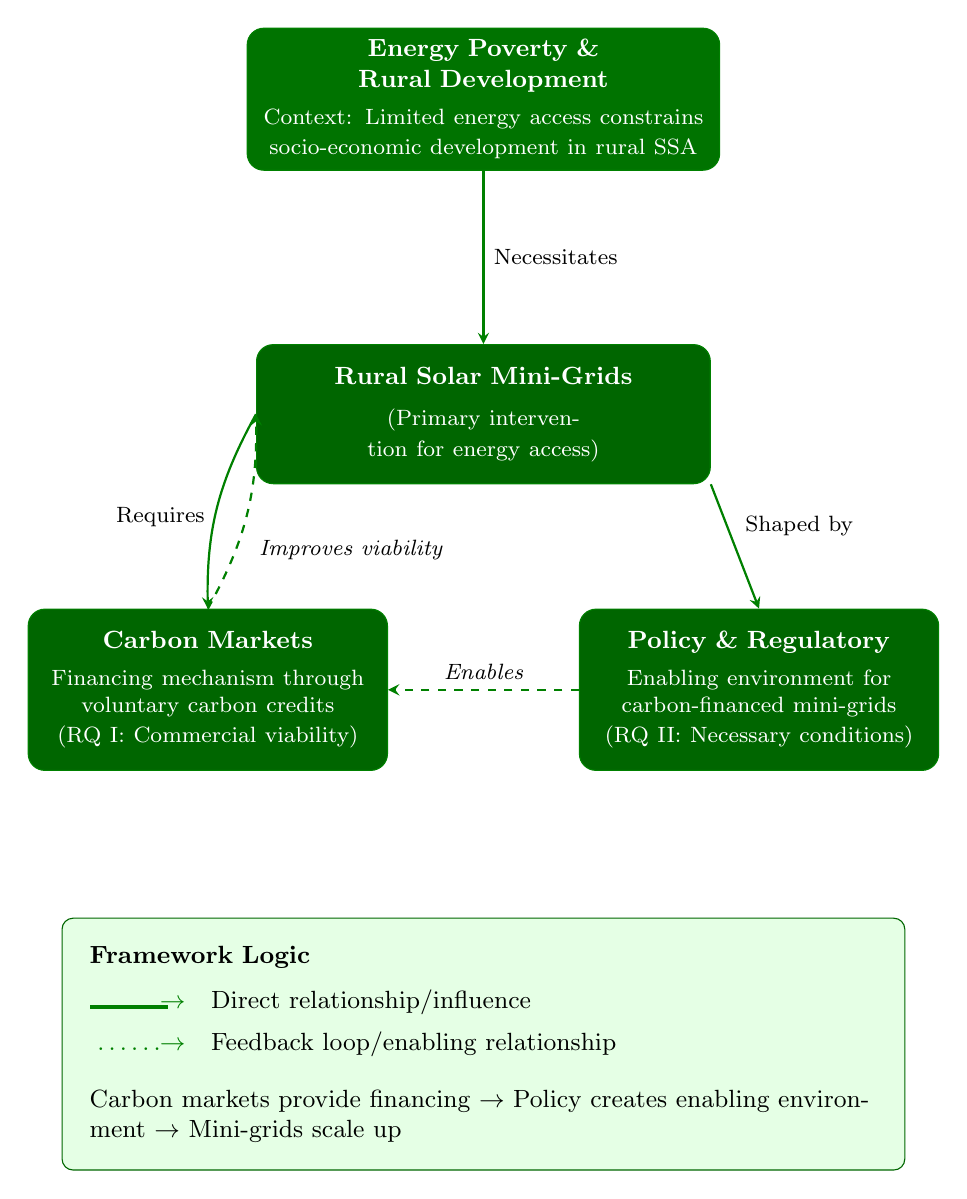
\begin{tikzpicture}[
  every node/.style={font=\small},
  topbox/.style={
    rectangle, rounded corners=6pt,
    draw=green!50!black, fill=green!45!black,
    text=white, text width=6cm, align=center,
    minimum height=1.4cm, inner xsep=0pt, inner ysep=4pt
  },
  mainbox/.style={
    rectangle, rounded corners=6pt,
    draw=green!50!black, fill=green!40!black,
    text=white, text width=5.2cm, align=center,
    minimum height=1.4cm, inner sep=8pt
  },
  sidebox/.style={
    rectangle, rounded corners=6pt,
    draw=green!50!black, fill=green!40!black,
    text=white, text width=4.0cm, align=center,
    minimum height=2.0cm, inner sep=8pt
  },
  legendbox/.style={
    rectangle, rounded corners=4pt,
    draw=green!40!black, fill=green!10,
    text=black, text width=10cm, align=left,
    inner sep=10pt
  },
  solidarrow/.style={
    ->, >=stealth, thick, green!50!black
  },
  dasharrow/.style={
    ->, >=stealth, thick, dashed, green!50!black
  },
]

% --- Nodes ---
\node[topbox] (poverty) at (0, 7.5)
  {\textbf{Energy Poverty \& Rural Development}\\[4pt]
   \footnotesize Context: Limited energy access constrains\\socio-economic development in rural SSA};

\node[mainbox] (minigrids) at (0, 3.5)
  {\textbf{Rural Solar Mini-Grids}\\[4pt]
   \footnotesize (Primary intervention for energy access)};

\node[sidebox] (carbon) at (-3.5, 0)
  {\textbf{Carbon Markets}\\[4pt]
   \footnotesize Financing mechanism through voluntary carbon credits\\(RQ I: Commercial viability)};

\node[sidebox] (policy) at (3.5, 0)
  {\textbf{Policy \& Regulatory}\\[4pt]
   \footnotesize Enabling environment for carbon-financed mini-grids\\(RQ II: Necessary conditions)};

% --- Solid arrows ---
% Necessitates: poverty -> minigrids
\draw[solidarrow] (poverty.south) -- node[right, text=black]{\footnotesize Necessitates} (minigrids.north);

% Shaped by: minigrids -> policy
\draw[solidarrow] (minigrids.south east) -- node[above right, text=black]{\footnotesize Shaped by} (policy.north);

% Requires: minigrids -> carbon (solid, outer arc bowing left/west)
\draw[solidarrow] (minigrids.west)
  to[bend right=15]
  node[left, pos=0.55, text=black, font=\footnotesize]{Requires}
  (carbon.north);

% --- Dashed arrows ---
% Improves viability: carbon -> minigrids (dashed, inner arc bowing right/east)
\draw[dasharrow] (carbon.north)
  to[bend right=15]
  node[right, pos=0.55, yshift=-16pt, text=black, font=\footnotesize\itshape]{Improves viability}
  (minigrids.west);

% Enables: policy -> carbon
\draw[dasharrow] (policy.west)
  -- node[above, text=black, font=\footnotesize\itshape]{Enables}
  (carbon.east);

% --- Legend ---
\node[legendbox] at (0, -4.5) {
  \textbf{Framework Logic}\\[6pt]
  \begin{tabular}{@{}l@{\quad}l@{}}
    {\color{green!50!black}\rule{1cm}{1.5pt}$\!\!\rightarrow$} & Direct relationship/influence \\[4pt]
    {\color{green!50!black}\makebox[1cm]{\dotfill}$\!\!\rightarrow$} & Feedback loop/enabling relationship \\[6pt]
  \end{tabular}\\[4pt]
  Carbon markets provide financing $\rightarrow$ Policy creates enabling environment $\rightarrow$ Mini-grids scale up
};

\end{tikzpicture}
\caption{Conceptual framework linking energy poverty, rural solar mini-grids, carbon markets, and policy.}
\label{fig:concept}
\end{figure}

The conceptual framework examines how carbon markets can support rural solar mini-grid deployment in SSA through interconnected components.

\begin{enumerate}
	\item \textbf{Carbon markets} as a financing mechanism, where voluntary credits can improve commercial viability but face uncertainties around transaction costs and certification, host government authorization, and revenue leakage to intermediaries.~\cite{kreibich2021,michaelowa-evolution,ahonen-governance}
	\item \textbf{Policy, regulatory, financial and technical frameworks,} which shape enabling conditions but often lack integration between energy regulations and carbon mechanisms, particularly regarding Article 6 authorization requirements and carbon revenue treatment within tariff structures.~\cite{esmap2019,bhattacharyya2016,schneider-integrity}
\end{enumerate}

Feedback loops link these components: regulatory clarity facilitates carbon market participation, and carbon finance strengthens commercial viability, enabling larger-scale projects. The framework guides investigation of barriers and enabling conditions across both RQs, with particular attention to structural market failures that prevent aggregation mechanisms from emerging organically.

\section{Methods}
\label{sec:methods}
We address these questions through stakeholder interviews, transaction cost analysis, and a case study of the atmosfair-MiniGridCo PoAs in Nigeria.

\subsection{Research Design}
\label{subsec:design}
This study employs a qualitative research design using thematic analysis~\cite{BraunClarke} to investigate how voluntary carbon markets support rural solar mini-grid development in SSA. Compliance markets were excluded to maintain scope clarity. Qualitative approaches are particularly suited for exploring emerging carbon market applications where empirical data are scarce~\cite{CreswellPoth} and for generating theoretically grounded insights into structural barriers and enabling conditions.~\cite{Flyvbjerg}

Given limited empirical evidence on carbon-financed mini-grids in SSA (Section~\ref{subsec:problem}), the research adopts an exploratory approach focused on identifying conditions, barriers, and stakeholder experiences. The study examines carbon market integration across Kenya and Nigeria, selected to capture variation in regulatory frameworks, operational scales, and institutional arrangements. Rather than treating these as comparative cases, the analysis seeks patterns across contexts along three analytical dimensions: stakeholder type (developers, carbon experts, policy officials, registry professionals); carbon finance engagement level (pursuing, attempted, rejected); and project scale (predominantly 100--500~kWp).

This cross-cutting approach enables identification of themes recurring across multiple settings, including regulatory clarity, institutional capacity, aggregation mechanisms, and transaction cost economics, addressing two research questions: (RQ1) on commercial viability and (RQ2) on necessary conditions for integration at scale.

\textbf{Positionality:} The lead researcher brings professional experience in development finance and environmental assessment in SSA, providing contextual familiarity with regulatory frameworks and project economics. This proximity enhanced interpretive depth but required reflexive awareness of potential confirmation bias toward structural explanations, managed through an analytical journal maintained throughout the study.

\textbf{Limitations:} This qualitative design provides rich insights into conditions and barriers but does not establish causality or quantify impacts. Findings should be interpreted as preliminary identification of structural factors requiring validation through larger-scale quantitative research.

\subsection{Study Sites and Case Selection}
\label{subsec:site-selection}
Kenya and Nigeria were selected as illustrative contexts rather than comparative cases. Kenya has relatively advanced regulatory frameworks (e.g., the Energy Act of 2019 and the Carbon Markets Regulations of 2024) with 150 Kenya Off-Grid Solar Access Project (KOSAP)-deployed mini-grids but minimal carbon-financed activity, a gap that is itself analytically significant given its institutional development. Nigeria hosts approximately 200 mini-grids~\cite{rea2025} and includes the atmosfair-MiniGridCo PoA, one of the few operational carbon-financed frameworks in SSA, providing a critical case for examining aggregation feasibility.

Developer portfolios ranged from 16~kWp to 1~MWp, predominantly 100--500~kWp, reflecting the prevalence of small-to-medium scale mini-grids in SSA and enabling analysis of scale-dependent barriers such as transaction costs, methodological suitability, and revenue potential. 

\subsection{Data Collection}
This study received ethical approval from the SOAS University of London Research Ethics Panel, granted by the CeDEP Dissertation Convenor on 7 April 2025. Data collection combined semi-structured interviews and document analysis. Data were collected between June and August 2025.

\subsubsection{Semi-Structured Interviews}
\label{subsec:interviews}
Table~\ref{tab:participants} details the nine semi-structured interviews conducted with stakeholders spanning developers, carbon market experts, policy and regulatory officials, and registry professionals.

\begin{table}[t]
	\centering
	\resizebox{\textwidth}{!}{%
	\begin{tabular}{l c c c c}
		\toprule
		\textbf{Code} & \textbf{Stakeholder Type} & \textbf{Organization Type} & \textbf{Region} & \textbf{Duration} \\
		\midrule
		\textbf{DEV-KE-01} & Developer & Private sector & SSA & 45 min. \\
		\textbf{DEV-KE-02} & Developer & Private sector & SSA & 50 min. \\
		\textbf{DEV-NG-01} & Developer & Private sector & SSA & 35 min. \\
		\textbf{DEV-NG-02} & Developer & Private sector & SSA & 48 min. \\
		\textbf{EXP-01} & Carbon expert & Investor and Consultant & International & 60 min. \\
		\textbf{EXP-02} & Carbon expert & Carbon Marketplace & International & 38 min. \\
		\textbf{POL-01} & Regulatory policy expert & Regional professional & SSA & 45 min. \\
		\textbf{POL-02} & Regulatory policy expert & Regional professional & SSA & 45 min. \\
		\textbf{REG-01} & Registry expert & Gold Standard, ex-Verra & International & 75 min. \\
		\bottomrule
	\end{tabular}}%
	\caption{\textbf{Overview of Interview Participants.} All interviews conducted via virtual meetings.}
	\label{tab:participants}
\end{table}

Participants were contacted through multiple channels. Developers were identified through industry associations, including the Alliance for Rural Electrification, Gold Standard Registry, and snowball referrals.~\cite{bryman2016} Policymakers and carbon experts were approached through professional social media channels (e.g., LinkedIn) by analysing their experience relevance to the study. The carbon registry official was recruited via direct contact with the organization's technical team. Attempts to engage additional representatives from development finance institutions and consulting firms were unsuccessful within the research timeframe, limiting perspectives from investment and technical advisory communities.

\subsubsection{Document Analysis and Quantitative Data}
\label{subsec:doc-analysis}
Quantitative data were obtained from PoAs publicly available on the Gold Standard Registry, carbon certification cost data compiled from Gold Standard and Verra fee schedules and expert interviews, and project capital cost data obtained from developers and verified against the Africa Minigrid Developers Association (AMDA)~\cite{amda-bam} regional benchmarks. These secondary data provide contextual insight and should be considered indicative rather than precise measurements.

\subsection{Data Analysis}
\label{subsec:analysis}
Thematic analysis followed Braun and Clarke's~\cite{BraunClarke} six-phase framework, with coding conducted by the lead author consistent with reflexive thematic analysis principles.~\cite{BraunClarke2019} Data capture varied by participant consent: recorded interviews were transcribed verbatim, while non-recorded interviews were documented through structured notes capturing key themes and direct quotes where possible. All data were coded inductively in a structured Excel workbook tracking participant, extract, initial code, emerging theme, and research question alignment, enabling systematic cross-participant comparison and iterative refinement.~\cite{saldana}

Trustworthiness rested primarily on multi-source convergence: key themes were tested across nine interviews spanning four stakeholder types and documentary evidence. The transaction cost barrier, for example, emerged independently from developer interviews, was corroborated by expert assessment, confirmed by registry fee schedule analysis, and validated by Power Africa revenue leakage data.~\cite{power-africa-credits} An analytical journal tracked interpretive decisions throughout, and coding decisions were reviewed by the dissertation supervisor on a sample of transcripts. Negative cases were examined systematically. For instance, DEV-KE-01's projection of meaningful carbon revenues at scale qualified the transaction cost theme as scale-dependent rather than absolute.
\section{Results and Discussion}
\label{sec:results}

\subsection{RQ1: How Effectively Do Carbon Finance Mechanisms Incentivize Investment and Improve Commercial Viability?}
\label{subsec:rq1}
Effectiveness was assessed through a combination of quantitative data (Section~\ref{subsec:doc-analysis}) and stakeholder perceptions, particularly from developers (Section~\ref{subsec:interviews}). This dual approach allowed for evaluation of how carbon market integration influences financial and operational outcomes in rural solar mini-grids in Kenya and Nigeria. Evidence is presented across these dimensions, highlighting both observed patterns and participant insights.

\subsubsection{Developer Perceptions of Carbon Market Viability}
Table~\ref{tab:awareness} details all four interviewed developers demonstrated awareness of carbon finance despite direct engagement remaining limited.

\begin{table}[h]
	\centering
	\resizebox{\textwidth}{!}{%
	\begin{tabular}{l l l l >{\raggedright\arraybackslash}p{4cm}}
		\hline
		\textbf{Developer} & \textbf{\makecell[lt]{Prior \\ awareness}} & \textbf{\makecell[lt]{Ever \\ considered}} & \textbf{\makecell[lt]{Current \\ status}} & \textbf{\makecell[lt]{Barrier/enabler \\ cited}} \\
		\hline
		\textbf{DEV-NG-01} & Yes, partial & Yes & Not pursuing & Complexity, high transaction costs, small project size \\
		\hline
		\textbf{DEV-NG-02} & Yes & Yes & Attempted & Low emission volumes, high costs, insuffiecient revenue \\
		\hline
		\textbf{DEV-KE-01} & Yes & No & Pursuing & Methodology challenges, high consultatn costs, small portfolio \\
		\hline
		\textbf{DEV-KE-02} & Yes & Yes & Pursuing & Market not accommodating, taxation, verification challenges \\
		\hline
	\end{tabular}}%
	\caption{Developer Awareness and Consideration of Carbon Finance}
	\label{tab:awareness}
\end{table}

Despite recognizing carbon revenue potential, none had successfully integrated carbon finance, with progress consistently constrained by project scale. Smaller mini-grids generate insufficient emissions reductions to justify transaction and monitoring costs, making carbon finance economically unviable. Several developers have opted for Renewable Energy Certificates (RECs) as simpler alternatives. DEV-NG-02 noted, ``Emissions to be avoided were relatively small, hence the transaction could not go through. It requires megawatts of energy projects.''

Expert perspectives reinforced structural barriers: "The cost of entry is high, and fragmentation is a big issue...methodologies weren't really designed with them in mind" (EXP-01). This aligns with Michaelowa et al.'s \cite{michaelowa-catalysing} finding that SSA was "essentially bypassed by the CDM," with only 22\% of single CDM projects and 16\% of PoA component activities issuing credits, a pattern this research confirms persists in voluntary markets.

\subsubsection{Transaction Costs and Certification Barriers}
Table~\ref{tab:costs} analyzes Gold Standard and Verra fee schedules, combined with developer-reported expenses, and reveals a multi-component cost structure creating significant cost barriers for mini-grid carbon certification.

\begin{table}
	\centering
	\resizebox{\textwidth}{!}{%
	\begin{tabular}{l l l l l}
		\hline
		\textbf{Cost Component} & \textbf{<200~kWp} & \textbf{200--500~kWp} & \textbf{>500~kWp} & \textbf{Source} \\
		\hline
		\textbf{Baseline study} & 4--5 & 10--20 & 20--40 & EXP-01, EXP-02 \\
		\hline
		\textbf{PoA registration} & 3.25--4.5 & 3.75--4 & 4--6 & \cite{goldStandardFees,verraFees} \\
		\hline
		\textbf{MRV system setup} & 15--25 & 35--40 & 40--60 & \cite{goldStandardFees,verraFees} \\
		\hline
		\textbf{15 annual verifications} & 18 & 30 & 30 & \cite{goldStandardFees,verraFees} \\
		\hline
		\textbf{Technical assistance} & 10--20 & 20--35 & 35--60 & DEV-KE-01, DEV-NG-02 \\
		\hline
		\textbf{Total} & 53--83 & 95--140 & 140--215 & Calculated totals \\
		\hline
	\end{tabular}}%
	\caption{\textbf{Carbon Certification Transaction Costs in thousands of USD.} Cost estimates compiled from carbon registry fee schedules,~\cite{goldStandardFees,verraFees} consultant expert interviews (EXP-01; EXP-02), and developer-reported project expenses (DEV-KE-01; DEV-NG-02). Verification costs calculated over typical 15-year project crediting period.}
	\label{tab:costs}
\end{table}

To assess the disproportionate burden of transaction costs on different project sizes, Table~\ref{tab:pct-costs} breaks down certification costs against typical mini-grid capital expenditure. CAPEX costs assume the average capital expenditure for mini-grids in SSA is approximately 6,824~USD/kWp.~\cite{amda-bam}

\begin{table}
	\centering
	\begin{tabular}{l r r r}
		\hline
		\textbf{\makecell[lt]{Project \\ Capacity}} & \textbf{\makecell[lt]{CAPEX \\ (kUSD)}} & \textbf{\makecell[lt]{Certification \\ Costs (kUSD)}} & \textbf{\% of CAPEX} \\
		\hline
		\textbf{100~kWp} & 682.4 & 68 & 10\% \\
		\hline
		\textbf{250~kWp} & 1,706 & 117.5 & 6.9\% \\
		\hline
		\textbf{500~kWp} & 3,412 & 177.5 & 5.2\% \\
		\hline
	\end{tabular}
	\caption{Transaction Costs as Percentage of Project CAPEX}
	\label{tab:pct-costs}
\end{table}

This analysis demonstrates that smaller projects face a higher relative burden of certification costs, underscoring the disproportionate impact of transaction costs on small-scale mini-grid developers. For mini-grids under 200~kWp, certification costs represent approximately 10\% of total capital expenditure, which developers consistently identified as a significant constraint on project feasibility. As one small developer noted, ``It requires megawatts of energy projects'' (DEV-NG-02).

Larger developers acknowledged certification costs but emphasized that operational and regulatory barriers often posed more substantial challenges: ``Mini-grids just aren't seen as a viable asset compared to cookstoves...aggregation would help, but it's not easy to pull off'' (EXP-01).

These perspectives indicate that, although transaction costs constitute a meaningful financial barrier, they interact with broader challenges, including project fragmentation, aggregation difficulties, and methodological complexities, that collectively limit the participation of smaller mini-grid developers in carbon markets.

\subsubsection{Revenue Projections}
Small-scale rural mini-grids face significant constraints generating carbon revenue due to limited scale and dispersed nature. As EXP-01 observed: ``Mini-grids just aren't seen as a viable asset.... Intermediaries and registries don't prioritize them because the returns are smaller.'' Current voluntary carbon market pricing of approximately 1--5 USD per \tcooe\ (EXP-02) renders transaction costs systematically greater than potential revenues for sub-200-kWp projects.

While PoA mechanisms theoretically allow small projects to pool credits across jurisdictions, achieving aggregation requires navigating complex registry requirements, demonstrating additionality, and coordinating operations, introducing substantial operational and financial challenges. As POL-02 noted, ``Aggregation is possible using programs of activities, but scalability is challenging because projects take years to join programs, and individual mini-grid volumes are low.'' Post-Paris governance fragmentation, with its competing standards, divergent accounting rules, and uncertain host government authorisation under Article 6, has further complicated the revenue outlook.~\cite{ahonen-governance}

These structural limitations underscore that small rural mini-grids cannot rely on carbon markets as meaningful revenue sources without aggregation mechanisms and supportive policy frameworks that current market structures do not produce organically.

\subsubsection{Summary of RQ1 Findings}
Carbon finance functions as a supplementary rather than transformative factor in mini-grid investment decisions. No developer indicated carbon revenue was decisive; instead, it is considered a ``nice-to-have'' addition to projects pursued independently of carbon finance opportunities. Transaction costs systematically exceed potential revenues for sub-megawatt projects, while revenue leakage means even successful credit sales deliver only a fraction of projected income to developers.~\cite{power-africa-credits}

While additionality is theoretically easier to demonstrate for mini-grids (i.e. projects often would not proceed without additional revenue), existing carbon methodologies were designed for larger-scale installations and require adaptation. Market realities of demand, pricing, and risk perception further constrain investor attention, with buyers not viewing mini-grids as strong asset classes compared to cookstoves or REDD+ projects.

Carbon finance can provide supplemental income but is insufficient as a primary investment incentive for mini-grids. Its impact on commercial viability depends on: (1) project aggregation to achieve economies of scale, (2) methodological adaptations to reduce transaction costs, (3) supportive policy frameworks to address regulatory barriers, (4) cross-border coordination enabling pooled credit volumes, and (5) resolution of post-Paris authorisation requirements under Article 6. Without these mechanisms, carbon finance acts as a secondary rather than standalone financial lever.

\subsection{RQ2: What Conditions Are Necessary for Successful Carbon Market Integration at Scale?}
\label{subsec:rq2}

\subsubsection{Technical Conditions}
MRV requirements present significant barriers for small-scale projects.~\cite{michaelowa2005} As EXP-01 noted: ``MRV is expensive, and the administrative burden is high. For small projects it just eats too much of the value.'' Many developers lack infrastructure and expertise for continuous emissions monitoring, while certifying bodies face knowledge gaps regarding mini-grid verification. Methodologies often consider embodied emissions from imported solar equipment, requiring supply chain tracking capacity that small operators lack (REG-01).

Establishing accurate baselines also proved challenging: ``Grid emission factors, were previously inflating the final emission reduction, so we have to go back and figure out how this reflects in different countries'' (REG-01).

Overcoming scale barriers requires aggregation, yet market mechanisms have failed to produce it organically. While Programme of Activities (PoA) mechanisms theoretically permit incremental project addition, they involve added complexity and scrutiny (REG-01). EXP-01 noted intermediaries focus on larger asset classes: ``If someone could aggregate projects under one umbrella and make it big enough, then maybe intermediaries would pay attention...but right now, they're focused on easier asset classes.''

The atmosfair-MiniGridCo PoA represents the sector's only significant success, succeeding due to four prerequisites absent for independent developers: specialized technical capacity, upfront capital absorbing the 35,000--65,000 USD certification costs, patient capital enabling 10+ year commitments, and registry credibility. Independent Nigerian developers (DEV-NG-01, DEV-NG-02) attempted carbon finance but failed.

Limited replication of the MiniGridCo model three years after its establishment is consistent with, though not conclusive proof of, structural market failure. The nascent timeframe means regulatory and awareness barriers may also be contributing factors. However, DEV-NG-01 and DEV-NG-02 both independently attempted and abandoned carbon finance, citing prohibitive costs and institutional barriers rather than awareness or timing, suggesting structural rather than transitional constraints. This is consistent with World Bank evidence that post-Paris carbon aggregation has become ``smaller, and less transparent, than during the Kyoto Protocol period.''~\cite{michaelowa-catalysing}

\subsubsection{Financial Conditions}
Transaction costs constitute the primary integration barrier. DEV-NG-02 reported: ``The volumes were too low and the revenue to be generated did not match up to the cost we would accrue for the registration and monitoring fees.'' Fixed auditor costs of 100,000--300,000 USD create minimum viable scale thresholds unattainable by individual mini-grids (REG-01).

Evidence on carbon revenue significance varies by project scale. DEV-KE-01 projected that carbon revenues could reach ``12--15\% of total revenue, close to 2 million euros a year once accredited'' for their portfolio. However, DEV-NG-02 reported that actual returns may fall below 5\% of total investment, indicating carbon revenue alone cannot salvage unviable projects. Carbon finance serves as a viability enhancer rather than primary solution, with its contribution depending heavily on project scale, aggregation success, and market pricing. Fundamental mismatches between investor expectations and mini-grid realities further constrain viability: ``Investors also want quick returns, but mini-grids are not a fast-moving business'' (DEV-NG-02).

\subsubsection{Regulatory and Policy Conditions}
POL-02 identified profound regulatory ambiguities in Kenya: ``There's no clear framework or harmonized registry for carbon credits.... Licensing for mini-grids is unclear, including whether developers should be regulated by the Central Bank or other agencies.'' This fragmentation creates uncertainty regarding project eligibility, credit ownership, and operational requirements.

Nigeria presents contrasting approaches. For projects under 1~MWp, ``you get a letter and start operations'' (DEV-NG-02), yet licensing pathway choice has substantive implications: ``If you do registration as a mini grid, you don't have this option [to be a generator]. If you do the permitting option, you can.'' POL-02 emphasized that ``power purchase agreements, leasing, and registration processes are ambiguous, especially for projects under 20 years,'' directly affecting carbon projects with 7--10 year crediting periods.

In Kenya, the Energy and Petroleum Regulatory Authority ``(EPRA) holds issuance of tariffs and approvals.... There is pressure to push tariffs down'' (DEV-KE-01), with stark variation across locations. The relationship between carbon revenues and tariff regulation remains undefined. If regulators treat carbon income as general project revenue, they may mandate tariff reductions, effectively capturing carbon revenues. Conversely, if treated as separate environmental benefit streams, developers retain them. POL-02 confirmed this ambiguity exists with no specific provisions. DEV-KE-01 described regulatory responsiveness challenges: ``Slow response, EPRA hasn't replied.... They are not ready and don't understand.''

REG-01 explained a critical barrier: ``Check [National Determined Contributions] (NDCs), say Kenya has claimed clean energy activity, your project is not additional.'' If governments include mini-grid deployment in unconditional NDC commitments, projects automatically fail additionality tests. POL-02 noted Kenya's experience with benefit-sharing requirements affecting Nature-Based Solutions projects. This creates perverse incentives: governments demonstrating climate ambition inadvertently disqualify domestic projects from carbon finance that could help achieve those targets, exemplifying the policy integration gap where energy and carbon market regulations operate in silos.

Post-Paris governance has intensified this challenge. Article 6.2 of the Paris Agreement requires host government authorization for internationally transferred mitigation outcomes (ITMOs), and host countries now ``bear an unprecedented task of ensuring the environmental integrity and robust accounting of ITMOs.''~\cite{ahonen-governance} Many SSA governments lack this capacity; Kenya has approved zero Article 6 projects despite its Climate Change Act (2016, amended 2023) and Carbon Markets Regulations (2024), which fix Corresponding Adjustment prices at USD 4 per \tcooe\ and strictly limiting Letters of Authorisation to preserve its carbon budget.

The consequences of this authorization barrier are severe. KOKO Networks, serving 1.5 million Kenyan households with bioethanol cooking fuel, entered administration in February 2026 after the Kenyan government refused a Letter of Authorisation, barring monetization under Article 6.2. Seven hundred employees lost jobs and 1.5 million households returned to charcoal and kerosene.~\cite{koko-disrupt} While KOKO Networks was not a mini-grid developer, this case directly validates the authorization risks identified in this research: even real, additional, verifiable emission reductions cannot succeed without host government authorization. The case illustrates the ``extreme fragility of business models that rely on the complex and often shifting regulatory landscapes of international carbon markets.''~\cite{koko-econews}

Grid arrival risk, which implies national grid extension reaching mini-grid areas, poses significant concerns for projects with 10--15-year carbon crediting periods. Nigeria's compensation framework pays ``the depreciated value plus one year of revenue'' (DEV-NG-02), failing to capture multi-year losses with no provision for lost carbon revenues, which one developer projected could reach 12--15\% of total revenue for larger portfolios. This creates fundamental incompatibility between carbon market requirements demonstrating permanence and multi-year monitoring commitments, and grid arrival policies that can unilaterally terminate these commitments.

In Kenya, carbon credit sales incur taxation between 25 and 40\%,~\cite{kenya-climate-change-regulations} substantially reducing net benefits. For example, DEV-KE-01's projected 12--15\% revenue contribution would decrease to approximately 9--11\% after taxation. POL-02 observed this ``discourages developers from selling credits locally,'' potentially incentivizing offshore sales. This taxation approach contradicts stated policy objectives. If carbon markets provide additional financing for marginal projects, taxing revenues at standard rates undermines additionality by capturing 25--40\% of the incremental benefits.

\subsubsection{Carbon Market-Specific Conditions}
Current carbon methodologies were not designed for mini-grids. Registries ``use CDM methodologies, they have been doing them for years'' (REG-01), but these originated for larger projects. Scale thresholds create barriers: projects above 60,000~\tcooe\ annually face stricter rules, while most individual mini-grids fall into microscale categories below 10,000~\tcooe. EXP-02 noted geographic aggregation precedents exist in regenerative agriculture but have not been systematically applied to renewable energy mini-grids. REG-01 confirmed ``registries are now designing for new RE and that is currently ongoing, decision made in 2023,'' indicating methodological adaptation is occurring but incomplete. The shift toward context-specific additionality assessment improves accuracy but increases complexity and transaction costs. The retroactive restriction proves particularly problematic: ``many projects have been running since 2011--2013, so they are not valid for carbon credits'' (DEV-KE-01), creating a chicken-and-egg financing problem.

Buyer preferences significantly shape viability. EXP-02 noted corporate buyers ``focus a lot on permanence'' and prefer removal over reduction credits, disadvantaging renewable energy projects. Recent price quotes ``around one U.S. dollar'' per \tcooe\ were described as ``ridiculous.'' Reputational risk aversion favors established project types, but mini-grids lack sufficient track record for rating agency assessment.

EXP-01 identified the fundamental issue: ``SSA will be a net seller, and the global north will be the buyers, that means the demand side decides what's acceptable.'' This power asymmetry means mini-grid viability depends on shifting buyer preferences in developed markets rather than demonstrating value to host country stakeholders.

Multiple respondents identified Renewable Energy Certificates as potentially more viable. REG-01 advised ``RECs are a safer choice, better regulated, less change and rules around them.'' DEV-KE-02 cited the R-REC Standard~\cite{rrecs} with ``methodology in line with UNFCCC guidelines that allows you to convert RECs to carbon credits,'' representing hybrid flexibility. Platform developments integrating ``I-RECs, TIGRs, and GEOs onto the same platform as carbon credits'' could increase liquidity (EXP-02). REG-01 noted D-RECs command premium prices ``because of their use in specialized areas'' like schools and clinics, suggesting co-benefit documentation enhances value.

EXP-02 described settlement innovations addressing transaction risks: ``We hold the credits...but they still remain the seller's, and then the buyer needs to transfer the money...two days for the payment to happen instead of 30.'' Platform neutrality and bank-grade requirements ensure trustworthy infrastructure, while multi-registry integration reduces transaction costs for buyers and sellers who previously needed separate accounts with each registry.

\subsubsection{Summary of RQ2 Findings}
Analysis reveals successful carbon market integration requires simultaneous convergence across five interdependent condition clusters. The atmosfair-MiniGridCo model's singular success alongside 200 other non-participating Nigerian mini-grids reveals a critical finding: aggregation mechanisms do not emerge organically from market forces.

The critical insight is MiniGridCo's limited replication is consistent with structural market inadequacy, corroborated by DEV-NG-01 and DEV-NG-02 citing prohibitive costs and institutional barriers rather than awareness or timing. Aggregation mechanisms do not emerge organically from market forces despite clear economic rationale and available PoA frameworks. This implies that without deliberate institutional intervention creating aggregation infrastructure, carbon finance remains inaccessible to the mini-grid sector regardless of individual developer capabilities or methodological improvements.

Three insights emerge:
\begin{enumerate}
	\item Market forces do not produce necessary aggregation infrastructure. MiniGridCo succeeded because atmosfair possesses institutional endowments, such as DFI backing, technical expertise, patient capital, unavailable to commercial developers, not because PoA mechanisms are accessible.
	\item Transaction cost economics remain prohibitive. Even with aggregation theoretically available, the existence of PoA pathways has not catalyzed adoption because upfront costs and complexity exceed independent developer capacity.
	\item Regulatory fragmentation creates structural incompatibilities that technical solutions alone cannot overcome, multiple policy domains must align simultaneously.
\end{enumerate}

Table~\ref{tab:rq2} synthesizes barriers and required changes, revealing that scale, aggregation, and transaction cost economics represent binding structural constraints rather than solvable technical problems. Addressing only one without the other yields insufficient improvement, while both depend on institutional capacity that current market structures do not produce.

\begin{table}
	\centering
	\resizebox{\textwidth}{!}{%
	\begin{tabular}{l >{\raggedright\arraybackslash}p{4cm} l >{\raggedright\arraybackslash}p{4cm} >{\raggedright\arraybackslash}p{4cm}}
		\hline
		\textbf{\makecell[lt]{Condition \\ domain}} & \textbf{Structural barrier} & \textbf{Priority} & \textbf{Dependencies} & \textbf{Required intervention} \\
		\textbf{\makecell[lt]{Scale and \\ aggregation}} & Individual projects economically unviable; PoA mechanisms exist but markets have not produced aggregation intermediaries despite 200+ mini-grids operating. & Critical & Requires institutional capacity that markets do not produce organically; depends on public or DFI support. & Establish publicly-funded aggregation intermediaries in SSA with mandate to absorb upfront costs and coordinate multi-developer PoAs. Market forces have proven insufficient. \\
		\hline
		\textbf{\makecell[lt]{Transaction \\ cost \\ economics}} & Fixed costs (100--300k USD) exceed small project revenues at 1--5 USD/\tcooe\ pricing. & Critical & Depends on aggregation and improved pricing. & Public subsidy of certification costs until scale achieved; registry fee waivers for aggregated projects; simplified MRV protocols requiring policy mandate. \\
		\hline
		\textbf{\makecell[lt]{Regulatory \\ framework}} & Carbon revenue treatment undefined in tariff regulations; grid arrival compensation excludes lost carbon revenues (potentially 12--15\% of income); 25--40\% taxation undermines additionality. & High & Enables project economics if combined with scale solutions. & Explicit carbon revenue provisions in licensing; tax exemptions or reduced rates. \\
		\hline
		\textbf{\makecell[lt]{Carbon \\ market \\ design}} & Methodologies designed for large projects; buyer preference for removal over reduction credits. & High & Requires registry willingness to adapt; influenced by buyer demand. & Mini-grid-specific methodologies with proportional MRV; REC-carbon hybrid instruments; revision of retroactive timeline restrictions; recognition of additionality in energy-poor contexts. \\
		\hline
		\textbf{\makecell[lt]{Institutional \\ capacity}} & No specialized intermediary serving mini-grid sector; registry access barriers for new entrants. & Medium & Becomes relevant only after critical constraints addressed; market has not produced this capacity organically. & Adoption of a mini-grid-specific standard to codify issuance rules, reduce verification overhead, and enable registry access via technical interoperability. \\
		\hline
	\end{tabular}}%
	\caption{Synthesis of Barriers and Required Interventions for Carbon Market Integration}
	\label{tab:rq2}
\end{table}

\subsection{Research Limitations}
This qualitative study provides empirically grounded insights but has several scope and generalizability constraints.
\begin{itemize}
	\item \textbf{Sample size and selection:} Four developers (4 of 7 contacted) provide depth but limit generalizability, with potential selection bias toward carbon-engaged developers. Absence of DFI perspectives constrains understanding of investment decision-making. Claims about scale conditions require validation through larger quantitative research.
	\item \textbf{Geographic specificity:} Findings reflect Kenya's and Nigeria's regulatory frameworks and are not directly generalizable to different policy environments.
	\item \textbf{Financial data precision:} Transaction cost analysis combines registry schedules, developer reports, and industry estimates without independent audit. Revenue projections involve uncertainty from future prices and demand.
	\item \textbf{Temporal context:} Data collection (June--August 2025) during carbon market transition. Registry methodology revisions incomplete; 1 USD/\tcooe\ pricing reflects research-time conditions.
\end{itemize}

Despite these limitations, multi-stakeholder design and cross-country comparison provide robust empirical evidence where such research remains scarce.
\section{Conclusions and Recommendations}
\label{sec:conc}

\subsection{Key Findings}
This research examined carbon markets' potential for supporting rural solar mini-grids in SSA through investigation of commercial viability and integration conditions. Evidence from four developers, five experts and policy officials, and one registry professional across Kenya and Nigeria reveals fundamental structural barriers limiting carbon finance effectiveness.

\textbf{Commercial Viability (RQ1):} Carbon finance functions as supplementary rather than transformative for mini-grid investments. No developer indicated carbon revenue was decisive. For projects under 200~kWp, certification costs represent approximately 10\% of CAPEX (Table \ref{tab:pct-costs}), while fixed auditing costs (100,000--300,000 USD) create minimum scale thresholds individual mini-grids cannot meet (REG-01). Current market pricing of 1--5 USD per \tcooe\ renders transaction costs systematically greater than potential revenues, consistent with transaction cost economics literature.~\cite{michaelowa2005,bellassen}

\textbf{Integration Conditions (RQ2):} Successful integration requires simultaneous convergence across five interdependent domains: technical capacity, financial viability, regulatory frameworks, institutional arrangements, and carbon market design. The atmosfair-MiniGridCo case provides evidence consistent with structural market inadequacy: despite technical success, MiniGridCo has not been replicated across 200+ other Nigerian mini-grids. This reveals that the conditions underlying MiniGridCo, specialized intermediary capacity, absorbed certification costs, patient capital, and registry credibility, are structurally unavailable to typical developers. Post-Paris governance fragmentation~\cite{ahonen-governance} and host government authorization requirements under Article 6 create additional barriers beyond those identified in pre-Paris literature. The February 2026 collapse of KOKO Networks following Kenya's refusal of a Letter of Authorisation~\cite{koko-disrupt} validates the authorization risks this research identified empirically, demonstrating these are not theoretical concerns but active threats to carbon-dependent business models.

\subsection{Implications}
\textbf{For Theory:} This research reveals an additionality paradox: projects with clearest need for additional financing face systematic exclusion due to transaction costs rather than failing additionality criteria.~\cite{michaelowa-evolution} Small mini-grids in remote areas would not proceed without carbon revenue, yet these characteristics create prohibitive certification costs, inverting carbon markets' stated purpose.

The MiniGridCo case illustrates market failure dynamics consistent with institutional economics on coordination problems and public goods provision: aggregation creates collective value but requires institutional capacity that individual actors cannot provide and markets do not produce organically. This confirms carbon market access for small-scale distributed renewable energy requires public sector intervention rather than purely market-based solutions.~\cite{michaelowa2005}

\textbf{For Policy:} Policymakers in Kenya and Nigeria face immediate decisions regarding carbon market integration. Current frameworks operate in silos, with energy regulations~\cite{epra-minigrid-regulations,nerc-minigrid-regulations} and carbon market frameworks~\cite{kenya-climate-change-regulations,ng-carbon-market-policy} lacking coordination. Three critical gaps require attention: (1) clarify carbon revenue treatment in tariff regulations, (2) reform grid arrival compensation to include lost carbon revenues, and (3) distinguish conditional from unconditional NDC targets to avoid disqualifying projects.~\cite{paris}

\textbf{For Practice:} Mini-grid developers should pursue carbon finance only within established aggregation programs, for projects exceeding 500~kWp, or with technical assistance covering certification costs. Independent small-scale developers face structural barriers that individual effort cannot overcome. Alternative mechanisms such as RECs may offer more accessible pathways (REG-01; DEV-KE-02). Carbon registries should develop mini-grid-specific methodologies with proportional MRV requirements and streamline PoAs registration.~\cite{goldStandardFees,verraFees,rrecs}

\subsection{Recommendations}
Successful carbon market integration for mini-grids requires coordinated interventions across multiple domains simultaneously. Priority actions include:

\noindent\textbf{Critical Infrastructure (Public Sector/DFI-Led):}
\begin{enumerate}
    \item Establish publicly-funded aggregation intermediaries in SSA with mandates to absorb upfront certification costs, provide technical support, and coordinate multi-developer PoAs. Market forces have proven insufficient to produce this infrastructure organically.
    \item Subsidize certification costs for aggregated renewable energy projects with registry fee waivers and simplified MRV protocols. DFIs should establish dedicated carbon market access facilities within rural electrification programs.
\end{enumerate}

\noindent\textbf{Regulatory Framework Reforms:}
\begin{enumerate}[resume]
    \item Issue explicit regulatory guidance on carbon revenue treatment within tariff frameworks (e.g., EPRA and the Nigerian Electricity Regulatory Commission, NERC), ensuring environmental benefit streams are not captured through mandatory tariff reductions.
    \item Reform grid arrival compensation frameworks to include projected carbon revenues over remaining crediting periods.~\cite{tenenbaum2014}
    \item Implement tax exemptions for carbon credit revenues to align with renewable energy policy objectives, and establish formal NDC-carbon market coordination distinguishing conditional from unconditional targets.~\cite{glasgow}
\end{enumerate}

\noindent\textbf{Carbon Market Design Adaptations:}
\begin{enumerate}[resume]
    \item Develop mini-grid-specific methodologies acknowledging bundled development co-benefits, proportional MRV requirements for microscale projects (<10,000~\tcooe\ annually), and strong additionality in energy-poor contexts.
    \item Create REC-carbon hybrid instruments providing diversified revenue streams~\cite{rrecs}.
\end{enumerate}

\noindent\textbf{Regional Coordination:}
\begin{enumerate}[resume]
    \item Develop harmonized carbon market frameworks through regional bodies (e.g., the East African Community, EAC, and the Economic Community of West African States, ECOWAS) enabling cross-border aggregation, similar to regional power pool coordination.~\cite{afdb2023}
    \item Integrate carbon finance realistically into national rural electrification master plans as supplementary rather than primary financing mechanism.
\end{enumerate}

\subsection{Future Research}
Three critical research gaps include:
\begin{enumerate}
    \item \textbf{Rigorous impact evaluation:} Quasi-experimental designs with baseline data, matched comparison groups, and longitudinal tracking (3--5 years) would enable robust causal inference on whether carbon finance affects tariffs, service quality, or community outcomes.~\cite{duflo} Key questions: Do carbon-financed projects serve more remote/lower-income communities? Does carbon revenue enable lower tariffs?
    \item \textbf{Financial performance analysis:} Detailed tracking of actual carbon revenue realization rates, timing relative to cash flow needs, audited transaction costs, and revenue volatility would address critical evidence gaps.~\cite{bhattacharyya2016} Understanding which project characteristics enable positive returns would inform targeting of carbon finance mechanisms.
    \item \textbf{Aggregation methods comparison:} Systematic comparison of aggregation models would identify optimal institutional arrangements balancing transaction cost reduction with developer autonomy and local ownership.
\end{enumerate}

\subsection{Conclusion}
This research demonstrates carbon markets face fundamental structural barriers limiting effectiveness for rural mini-grid financing in sub-Saharan Africa. Transaction costs systematically exceed potential revenues for small-scale projects. Methodologies inadequately address mini-grid characteristics. Regulatory frameworks fail to integrate carbon revenue considerations. Most critically, institutional intermediaries necessary for aggregation do not emerge organically from market forces, the atmosfair-MiniGridCo case demonstrates technical feasibility while demonstrating market inadequacy through non-replication.

Carbon market integration requires coordinated public intervention across all five condition domains simultaneously (Table~\ref{tab:rq2}). Addressing single constraints proves insufficient; systemic structural transformation is necessary. This includes publicly-funded aggregation infrastructure, regulatory reforms clarifying carbon revenue treatment, simplified methodologies with proportional MRV requirements, and regional coordination, interventions that markets alone will not produce.~\cite{michaelowa2005}

For the 600 million people in sub-Saharan Africa lacking electricity access,~\cite{iea2023} carbon markets represent one potential supplementary financing mechanism among many necessary tools. Grant finance, concessional loans, innovative business models, and supportive policies all play essential roles.~\cite{esmap2019,tenenbaum2014} Carbon finance can supplement these mechanisms under specific conditions requiring substantial institutional support, but expectations must be calibrated accordingly.

The imperative of universal energy access by 2030~\cite{un2030agenda} demands pragmatic assessment of what works, clear identification of what must change, and sustained commitment to ensuring climate finance mechanisms serve rather than constrain energy access goals. This research indicates that without major structural reforms, particularly publicly-funded aggregation infrastructure and regulatory framework integration, carbon markets will remain largely inaccessible to the mini-grid sector.

\appendix
\section{Interview Guides}
\label{app:interview-guides}

\subsection{Interview Guide 1: Mini-Grid Developers/Operators}
\textbf{Introduction}

Thank you for participating. This research examines how carbon markets can support rural mini-grid development in sub-Saharan Africa. Your insights on commercial viability, implementation experiences, and policy environments are valuable for understanding barriers and opportunities.

\textbf{Background}
\begin{enumerate}
	\item Can you describe your organization's mini-grid portfolio? (Number of sites, capacity, locations, business model)
	\item What are your biggest financing challenges for mini-grid projects?
\end{enumerate}

\textbf{B. Carbon Market Engagement}
(Use the relevant subsection based on respondent profile)
For developers pursuing / having pursued carbon credits:
\begin{enumerate}[resume]
	\item What motivated your organization to pursue carbon financing for mini-grids?
	\item Walk me through your experience with the carbon certification process. What were the key steps and challenges?
	\item How significant are carbon revenues relative to your overall project economics?
	\item What transaction costs did you encounter? (Financial, time, technical capacity)
	\item Did carbon credit requirements affect how you design or operate mini-grids?
\end{enumerate}

For developers who considered but rejected carbon finance:
\begin{enumerate}[start=3]
	\item What made your organization consider carbon financing initially?
	\item What factors led to the decision not to pursue carbon credits?
	\item What would need to change to make carbon markets viable for your projects?
\end{enumerate}

For developers who never seriously considered carbon finance:
\begin{enumerate}[start=3]
	\item Are you aware of carbon market opportunities for mini-grids?
	\item Why hasn't your organization pursued carbon financing?
	\item What concerns or barriers do you perceive regarding carbon markets?
\end{enumerate}

\textbf{C. Policy and Regulatory Environment}
\begin{enumerate}[start=8]
	\item How do current regulations in [Kenya/Nigeria] support or hinder mini-grid development?
	\item Are there specific policies affecting how carbon revenues would be treated? (Taxation, tariffs, subsidies)
	\item What regulatory changes would most help scale mini-grid deployment?
\end{enumerate}

\textbf{D. Development Impacts}
\begin{enumerate}[resume]
	\item What socio-economic benefits do your mini-grids deliver to communities?
	\item How do you balance financial sustainability with maximizing community benefits?
	\item If carbon revenues were available, how might they be used? (Lower tariffs, expand capacity, community programs)
\end{enumerate}

\textbf{E. Implementation Insights}
\begin{enumerate}[resume]
	\item What factors have been critical to your successful projects?
	\item What advice would you give other developers considering carbon finance?
\end{enumerate}

\subsection{Interview Guide 2: Policymakers/Regulators}
\textbf{Introduction}

Thank you for participating. This research examines policy frameworks that could enable carbon market integration with rural mini-grids. Your perspective on regulatory environments and policy development is essential.

\textbf{A. Policy Context}
\begin{enumerate}
	\item What are your country's/region's current priorities for rural electrification?
	\item How do mini-grids fit within national energy access strategies?
	\item What financing mechanisms currently support mini-grid development?
\end{enumerate}

\textbf{B. Carbon Market Integration}
\begin{enumerate}[resume]
	\item Is carbon financing for mini-grids discussed in policy circles? If so, how?
	\item Are there existing regulations addressing how carbon revenues should be treated? (Taxation, tariff implications, licensing requirements)
	\item What coordination exists between your ministry/agency and those responsible for climate/carbon policy?
\end{enumerate}

\textbf{C. Regulatory Gaps and Barriers}
\begin{enumerate}[resume]
	\item What policy gaps currently hinder mini-grid deployment generally?
	\item What specific regulatory challenges would carbon-financed mini-grids face?
	\item How do current policies address project aggregation across multiple developers?
\end{enumerate}

\textbf{D. Enabling Environment}
\begin{enumerate}[resume]
	\item What policy changes could facilitate carbon market integration with mini-grids?
	\item What institutional capacity would be needed to implement such policies?
	\item Are there concerns about carbon financing potentially conflicting with other policy objectives? (Tariff affordability, subsidy programs, grid extension plans)
\end{enumerate}

\textbf{E. Regional Cooperation}
\begin{enumerate}[resume]
	\item What regional initiatives could support carbon-financed mini-grid development?
	\item What lessons from other countries might be applicable here?
\end{enumerate}

\textbf{F. Future Directions}
\begin{enumerate}[resume]
	\item How do you see the role of carbon markets in achieving electrification targets?
\end{enumerate}

\subsection{Interview Guide 3: Carbon Registry Official/Methodologist}
\textbf{Introduction}

Thank you for participating. This research examines barriers and opportunities for integrating carbon markets with rural mini-grids in sub-Saharan Africa. Your expertise on methodologies and certification processes is invaluable.

\textbf{A. Methodology and Standards}
\begin{enumerate}
	\item What methodologies does [Gold Standard/Verra] offer for mini-grid projects?
	\item How do these methodologies account for mini-grid characteristics? (Small scale, rural contexts, limited baseline data)
	\item What are typical certification timelines and costs for mini-grid projects?
\end{enumerate}

\textbf{B. Developer Engagement}
\begin{enumerate}[resume]
	\item What level of interest have you observed from mini-grid developers in sub-Saharan Africa?
	\item What barriers do developers most commonly face in pursuing certification?
	\item How does project scale affect certification feasibility?
\end{enumerate}

\textbf{C. Aggregation Mechanisms}
\begin{enumerate}[resume]
	\item Can you explain how Programme of Activities (PoA) or grouped project approaches work for mini-grids?
	\item What are the requirements and costs for establishing a PoA?
	\item Why has uptake of aggregation mechanisms been limited in the mini-grid sector?
\end{enumerate}

\textbf{D. Co-Benefits and Impact Measurement}
\begin{enumerate}[resume]
	\item How do current methodologies value development co-benefits beyond emission reductions? (Health, education, gender impacts)
	\item Are there discussions about enhancing co-benefit recognition in mini-grid methodologies?
\end{enumerate}

\textbf{E. Transaction Costs and Streamlining}
\begin{enumerate}[resume]
	\item What efforts are underway to reduce transaction costs for small-scale projects?
	\item Could digital monitoring or simplified verification approaches reduce costs?
\end{enumerate}

\textbf{F. Market Dynamics}
\begin{enumerate}[resume]
	\item How do you see voluntary carbon market demand for mini-grid projects?
	\item What advice would you give mini-grid developers considering carbon certification?
\end{enumerate}

\subsection{Interview Guide 4: Carbon Experts}
\textbf{Introduction}

Thank you for participating. This research examines how carbon markets can support rural mini-grid deployment in sub-Saharan Africa. Your expertise in carbon finance and project development provides valuable perspective on implementation realities.

\textbf{A. Carbon Market Landscape}
\begin{enumerate}
	\item How would you characterize the current state of carbon markets for small-scale renewable energy projects in sub-Saharan Africa?
	\item What types of renewable energy projects are successfully accessing carbon finance in the region?
\end{enumerate}

\textbf{B. Mini-Grid Specific Challenges}
\begin{enumerate}[resume]
	\item What are the primary barriers preventing mini-grid developers from accessing carbon markets?
	\item How do transaction costs for mini-grid carbon certification compare to project revenues?
	\item At what project scale do carbon economics become viable for mini-grids?
\end{enumerate}

\textbf{C. Implementation Experience}
\begin{enumerate}[resume]
	\item Have you worked with or observed mini-grid carbon projects in Africa? What were the key success factors or failure points?
	\item What role do intermediaries or aggregators play, and why aren't there more serving the mini-grid sector?
\end{enumerate}

\textbf{D. Methodological and Technical Issues}
\begin{enumerate}[resume]
	\item Are current carbon methodologies well-suited to mini-grid contexts, or do they need adaptation?
	\item What are the biggest technical challenges for mini-grids in meeting MRV requirements?
\end{enumerate}

\textbf{E. Market Access and Pricing}
\begin{enumerate}[resume]
	\item How do voluntary carbon buyers view mini-grid credits compared to other project types?
	\item What's the pricing differential?
\end{enumerate}

\subsection{Ethical Considerations}
\begin{itemize}
	\item Obtain informed consent before beginning
	\item Remind participants they can skip questions or stop anytime
	\item Ensure confidentiality and explain how data will be used
	\item Provide contact information for follow-up questions
\end{itemize}
\section{Research Participant Information Sheet Template}
\label{app:info-sheet}

\textbf{Introduction}

The purpose of this form is to provide you with information, so you can decide whether to participate in this study. Any questions you may have will be answered by the researcher or by the other contact persons provided below. Once you are familiar with the information on this sheet and have asked any questions you may have, you can decide whether or not to participate. If you agree, you will be asked to fill in the consent form for this study or record your consent verbally.

\begin{longtable}{>{\raggedright\arraybackslash}p{0.28\linewidth} >{\raggedright\arraybackslash}p{0.65\linewidth}}
		\hline
		\textbf{\makecell[lt]{Research \\ title}} & Leveraging Carbon Markets to Scale Up Rural Solar Mini Grids and Accelerate Sustainable Development in Sub-Saharan Africa. \textbf{Alternative Title:} How carbon finance can help fund rural electricity projects in Africa. \\
		\hline
		\textbf{\makecell[lt]{Name and contact \\ details of \\ researcher}} & Name: Flora Aluoch Oloo Email: 684134@soas.ac.uk or floraoloo24@gmail.com \\
		\hline
		\textbf{\makecell[lt]{Name and contact \\ details of Principal \\ Investigator}} & Supervisor: Anabelle De Freece Email: af12@soas.ac.uk \\
		\hline
		\textbf{\makecell[lt]{What type of \\ research project is \\ this?}} & Non-Funded Research Project \\
		\hline
		\textbf{\makecell[lt]{Who is funding \\ this research \\ project?}} & Self-funded Masters Research Project \\
		\hline
		\textbf{\makecell[lt]{Who else is \\ involved with the \\ research project?}} & This research is conducted solely by the researcher at SOAS University of London. No other organizations have access to the data collected, though anonymized findings may be shared with development organizations and policy makers to inform practice. \\
		\hline
		\textbf{\makecell[lt]{What is the \\ research project's \\ purposes?}} & Many rural communities in Sub-Saharan Africa lack access to electricity, which limits economic development and quality of life. At the same time, there are financing challenges that make it difficult to build solar mini-grids in these communities. This research explores whether carbon markets could help finance more rural electricity projects. The study aims to understand the opportunities and barriers for using carbon finance to scale up rural solar mini-grids, assess the potential benefits for communities, and identify what policies would make this approach successful. \\
		\hline
		\textbf{\makecell[lt]{Why have I been \\ chosen?}} & You have been selected because of your expertise and experience in solar mini-grid development and rural electrification in Sub-Saharan Africa. Your insights are valuable for understanding how carbon finance could work in practice for rural electrification projects. Participants in the research projects cut across different stakeholder groups including developers, policy makers, investors, and community members. \\
		\hline
		\textbf{\makecell[lt]{Do I have to take \\ part?}} & Participation in this research is entirely voluntary. You can choose not to answer any questions you're uncomfortable with, or withdraw from the study at any time without giving a reason. If you withdraw, any data you have provided will be deleted unless you specifically agree to its continued use. \\
		\hline
		\textbf{\makecell[lt]{What will happen \\ to me if I take \\ part?}} & You will participate in a 30--45-minute interview (in-person, by phone, or video call) where I will ask about your experiences, perspectives, and opinions on carbon finance and mini-grid development. Questions will cover topics like financing challenges, carbon market mechanisms, policy frameworks, and community impacts. \\
		\hline
		\textbf{\makecell[lt]{Will I be recorded \\ and how will the \\ recordings be \\ used?}} & With your permission, interviews will be audio recorded to ensure accurate data collection. Recordings will only be used for research analysis and will be transcribed by the researcher or a professional transcription service bound by confidentiality agreements. Video recording will only be used if the interview is conducted online and you consent. \\
		\hline
		\textbf{\makecell[lt]{Risks and Benefits \\ of participation}} & \textbf{Benefits:}
		\begin{itemize}[noitemsep,topsep=2pt]
			\item Contributing to research that could help improve energy access in rural Africa
			\item Opportunity to share your expertise and influence policy recommendations
			\item Access to research findings that may inform your work
		\end{itemize}
		\textbf{Risks:}
		\begin{itemize}[noitemsep,topsep=2pt]
			\item Minimal risk beyond those of normal professional conversations
			\item Some questions may touch on business-sensitive topics, but you can decline to answer any question
			\item Time commitment required for participation
		\end{itemize}
		No direct financial benefits are provided for participation. \\
		\hline
		\textbf{\makecell[lt]{What if Something \\ Goes Wrong?}} & If you have concerns about any aspect of this research, please contact me directly using the details above. If you wish to make a formal complaint or have concerns that cannot be resolved through direct contact, you can contact Flora Aluoch Oloo 684134@soas.ac.uk or Anabelle De Freece Email: af12@soas.ac.uk \\
		\hline
		\textbf{\makecell[lt]{Where will \\ information I \\ proved be \\ transferred to?}} & Data will be collected in Kenya and Nigeria for analysis by the researcher at SOAS University of London. All data transfers will comply with international data protection standards. \\
		\hline
		\textbf{\makecell[lt]{How will \\ information I \\ provide be kept \\ secure?}} & Digital recordings and transcripts will be stored on password-protected, encrypted devices and physical documents used during community engagements will be kept in locked filing cabinets and shredded within 1 year of project completion. Only the researcher will have access to identifiable data. \\
		\hline
		\textbf{\makecell[lt]{Will I be kept \\ anonymous in this \\ research project?}} & Yes, you will be anonymized in all research outputs. Steps to protect your anonymity include: \begin{itemize}
			\item Removing names, organizations, and specific locations from transcripts and publications
			\item Using general descriptors (e.g., "mini-grid developer in East Africa" rather than specific company names)
			\item Aggregating data where possible to prevent identification
			\item Reviewing all quotes and examples to ensure they cannot be traced back to you
		\end{itemize} Note: Due to the small size of the mini-grid sector in some regions, complete anonymity cannot be guaranteed if you provide very specific details about unique projects or circumstances. You can indicate if any information should be treated as particularly sensitive. \\
		\hline
		\textbf{\makecell[lt]{What will happen \\ to the results of \\ this research \\ project?}} & Research results will be published in a Masters thesis (available through SOAS library and online repositories as well as academic journal articles). All published materials will maintain participant anonymity. You can request a summary of findings once the research is completed. The research aims to inform policy makers, development organizations, and practitioners working on rural electrification in Sub-Saharan Africa. \\
		\hline
\end{longtable}

\textbf{Data Protection Privacy Notice}

The data controller for this project will be SOAS University of London. The SOAS Data Protection Officer provides oversight of SOAS activities involving the processing of personal data and can be contacted at dataprotection@soas.ac.uk.

Your personal data will be processed for the purposes outlined in this Information Sheet. The legal basis that would be used to process your personal data under UK Data Protection Legislation is the performance of a task in the public interest or in our official authority as a controller. However, for ethical reasons we need your consent to take part in this research project. You can provide your consent for the use of your personal data in this project by completing the consent form that has been provided for you or via audio recording of the information sheet and consent form content.

\textbf{Your Rights}

You have the right to request access under the UK-GDPR to the information which SOAS holds about you. Further information about your rights under the Regulation and how SOAS handles personal data is available on the Data Protection pages of the SOAS website (\url{http://www.soas.ac.uk/infocomp/dpa/index.html}), and by contacting the Information Compliance Manager at the following address: Information Compliance Manager, SOAS, Thornhaugh Street, Russell Square, London WC1H 0XG, United Kingdom (e-mail to: dataprotection@soas.ac.uk).

If you are concerned about how your personal data is being processed, please contact SOAS In the first instance at dataprotection@soas.ac.uk. If you remain unsatisfied, you may wish to contact the Information Commissioner's Office (ICO). Contact details, and details of data subject rights, are available on the ICO website at: \url{https://ico.org.uk/for-organisations/data-protection-reform/overview-of-the-gdpr/individuals-rights/}

\textbf{Copyright Notice}

The consent form asks you to waive copyright so that SOAS and the researcher can edit, quote, disseminate, publish (by whatever means) your contribution to this research project in the manner described to you by the researcher during the consent process. 

\textbf{Contact for Further Information}

Name: Flora Aluoch Oloo Email: 684134@soas.ac.uk or floraoloo24@gmail.com

Thank you for reading this information sheet and for considering taking part in this research study.
\section{Sample Research Participant Consent Form Template}
\label{app:consent-form}
Consent Form for undertaking research on how carbon finance can help fund rural electricity projects in Africa and accelerate sustainable development in Sub-Saharan Africa

Please complete this form after you have read the Information Sheet and/or listened to an equivalent explanation about the research

\textbf{Project Title:} Leveraging Carbon Markets to Scale Up Rural Solar Mini Grids and Accelerate Sustainable Development in Sub-Saharan Africa.

\textbf{Researcher Name:} Flora Aluoch Oloo

\begin{longtable}{>{\raggedright\arraybackslash}p{0.8\linewidth} c c}
	\hline
	\textbf{Please tick the appropriate boxes} & \textbf{Yes} & \textbf{No} \\
	\hline
	I have read and understood the project information sheet dated 11 September 2025, or it has been read to me. & X & \\
	\hline
	I have been able to ask questions about the project & X & \\
	\hline
	I understand that potential risks of participating in this research include time commitment for interviews. & X & \\
	\hline
	I agree to take part in the project and understand that taking part involves participating in audio-recorded interviews lasting 30--45 minutes, or completing online surveys lasting 15--20 minutes, or participating in community focus group discussions. & X & \\
	\hline
	I agree that my interview is recorded on paper. & X & \\
	\hline
	I understand that I can refuse to answer questions & X & \\
	\hline
	I understand that my taking part is voluntary; I can withdraw from the study at any time by notifying the researcher/s involved and I do not have to give any reasons for why I no longer want to take part & X & \\
	\hline
	I understand that my withdrawal or refusal to take part will not affect my relationship with SOAS University of London or any organization I may be affiliated with. & X & \\
	\hline
	I understand that that personal information collected about me that can identify me, such as my name or where I live, will not be shared beyond the research team & X & \\
	\hline
	I understand information I provide will be stored securely by password-protected with access limited to the researcher only. & X & \\
	\hline
	I understand that the information I provided will be used for the MSc thesis, academic journal articles, policy reports, and other research outputs and made available through SOAS Research Online, academic publisher websites, and policy organization publications. & X & \\
	\hline
	I understand that my information will be anonymised so that I cannot be identified in the publications, reports, web pages, MSc thesis, and other research outputs, with names, organizations, and specific locations removed from all materials. & X & \\
	\hline
	I agree to waive copyright and other intellectual property rights in the material I contribute to the project & X & \\
	\hline
\end{longtable}

\textbf{Contact Information}

\textbf{Telephone No:} +254710885653

Email Address: 684134@soas.ac.uk

Postal Address: 22214-00100 Nairobi, Kenya

Alternative contact: Anabelle De Freece Email: af12@soas.ac.uk

\textbf{Research Participant Declaration}

I have accurately read out the information sheet to the potential participant and to the best of my ability, ensured that that participant understands what they are freely consenting.

\vspace{1.5em}
\begin{tabular}{p{0.45\linewidth} p{0.25\linewidth} p{0.2\linewidth}}
\rule{\linewidth}{0.4pt} & \rule{\linewidth}{0.4pt} & \rule{\linewidth}{0.4pt} \\
Name of Participant & Signature & Date \\
\end{tabular}

\vspace{1.5em}
\begin{tabular}{p{0.45\linewidth} p{0.25\linewidth} p{0.2\linewidth}}
\rule{\linewidth}{0.4pt} & \rule{\linewidth}{0.4pt} & \rule{\linewidth}{0.4pt} \\
Name of Researcher & Signature & Date \\
\end{tabular}

SOAS Consent Form Adapted From UK Data Archives Model Consent Form and licensed under the Creative Commons Attribution-Non-Commercial-Share-Alike 4.0 International Licence

\textbf{Please ensure a copy of this document is retained safely for future reference.}
\section{Sample Interview Transcript}
\label{app:transcript}
\textbf{Interviewer:} How would you characterize the current state of carbon markets for small-scale renewable energy projects in sub-Saharan Africa?

\textbf{EXP-01:} Investors are still more interested in bigger, grid-connected projects where excess power can be sold back to the grid. Rural mini grids don't attract the same kind of commercial attention. Impact funds are still commercially focused, even if their LPs are a bit more patient. There's this shift happening, DFIs like the British have scaled down grants and shifted to more commercial investments. It's becoming more of a trade-not-aid mentality.

\textbf{Interviewer:} What types of renewable energy projects are successfully accessing carbon finance in the region?

\textbf{EXP-01:} Mini-grids just aren't seen as a viable asset compared to things like cookstoves. Intermediaries and registries don't prioritize them because the returns are smaller. If someone could aggregate projects under one umbrella and make it big enough, then maybe intermediaries would pay attention, because they could earn higher fees. But right now, they're focused on easier asset classes.

\textbf{Interviewer:} What are the primary barriers preventing mini-grid developers from accessing carbon markets?

\textbf{EXP-01:} The cost of entry is high, and fragmentation is a big issue. These developers are small and scattered, and the methodologies weren't really designed with them in mind. Verra and Gold Standard dominate most of the market, like 80\%, so it's really their policies that matter. From a policy perspective, it's their rules you have to influence.

\textbf{Interviewer:} How do transaction costs for mini-grid carbon certification compare to project revenues?

\textbf{EXP-01:} Covering the MRV costs and registration links straight back to investor returns. If the transaction costs are too high compared to what you can earn in credits, then the economics just don't work. That's why people keep trying to aggregate across countries, but it's tough to pull off.

\textbf{Interviewer:} At what project scale do carbon economics become viable for mini-grids?

\textbf{EXP-01:} I don't have a number, but megawatt-scale projects obviously do better than small rural systems. Maybe mini-grids tied to hospitals or schools that can connect to the main grid would make more sense. Mini-grid financing has better additionality prospects, you can argue that without carbon revenues, these projects wouldn't happen.

\textbf{Interviewer:} Have you worked with or observed mini-grid carbon projects in Africa? What were the key success factors or failure points?

\textbf{EXP-01:} I've seen people trying to aggregate projects across different countries. That's the holy grail. But it's hard because of transaction costs, small size, and policy fragmentation. Permanence and additionality still matter the same way whether it's a large grid or a mini-grid. The concepts don't change, but how you account for them does.

\textbf{Interviewer:} What role do intermediaries or aggregators play and why aren't there more serving the mini-grid sector?

\textbf{EXP-01:} They're not interested commercially. Mini-grids aren't attractive enough compared to other assets like cookstoves. If someone could bring a big aggregated bundle of projects, then maybe. But intermediaries would also need to invest in defining new methodologies, and right now that's not worth it to them.

\textbf{Interviewer:} Are current carbon methodologies well-suited to mini-grid contexts, or do they need adaptation?

\textbf{EXP-01:} Methodologies are evolving because of integrity concerns. There's been so much noise about greenwashing that buyers and registries are tightening up. Additionality is actually easier to prove with mini-grids, because without carbon revenue they often wouldn't happen. But the methodologies weren't designed with them in mind, so they'd need tweaking.

\textbf{Interviewer:} What are the biggest technical challenges for mini-grids in meeting MRV requirements?

\textbf{EXP-01:} MRV is expensive, and the administrative burden is high. For small projects it just eats too much of the value. People think methodologies will get better over time, but who influences the registries? It's not governments. It's mostly the private sector on the demand side.

\textbf{Interviewer:} How do voluntary carbon buyers view mini-grid credits compared to other project types? What's the pricing differential?

\textbf{EXP-01:} Buyers don't see mini-grids as a strong asset class, especially compared to cookstoves or REDD+. They just don't think the returns justify the effort. SSA will be a net seller, and the global north will be the buyers, that means the demand side decides what's acceptable. There's also more reputational risk now about integrity and greenwashing, so buyers are cautious.

\textbf{Additional insights documented from EXP-01:}
\begin{itemize}
	\item There's interest in using instruments like green bonds, insurance products, or SPACs to derisk and bundle assets.
	\item Article 6 rules and integrity debates are reshaping how additionality and permanence are handled.
	\item Some markets like Zimbabwe or South Africa could have more viable mini-grid carbon projects because they're so coal-reliant.
	\item Rural mini-grid scalability is still viewed skeptically compared to other clean energy assets.
	\item Registries and demand-side actors, not governments, are likely to influence how methodologies evolve.
\end{itemize}
\clearpage
\section{Site imagery and information for Site A}
\label{app:site-imagery}
The Toto mini grid is a 352.24-kWp interconnected hybrid solar power plant in Toto, Nasarawa State, Nigeria, that provides reliable, renewable electricity to over 2,000 households and businesses, including the community's General Hospital.

\begin{figure}[h]
	\centering
	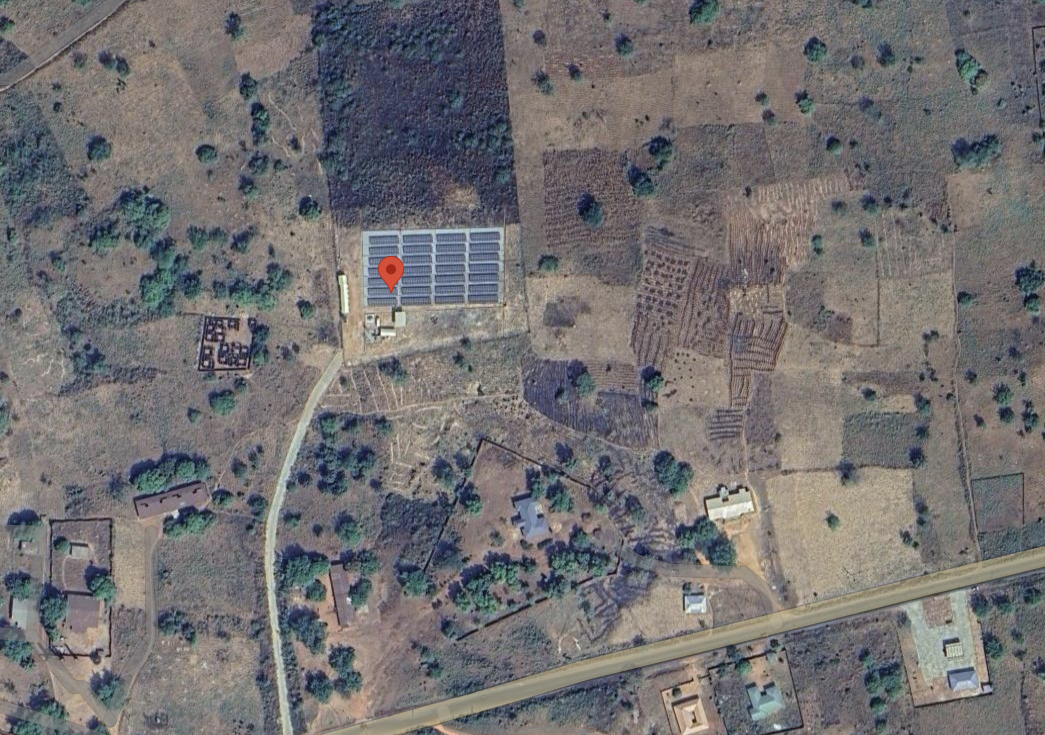
\includegraphics[width=0.6\textwidth]{figures/satellite.png}
	\caption{Toto Site Satellite Imagery: 8°23'39.0"N 7°05'20.9"E - Google Maps}
\end{figure}

\begin{figure}[h]
	\centering
	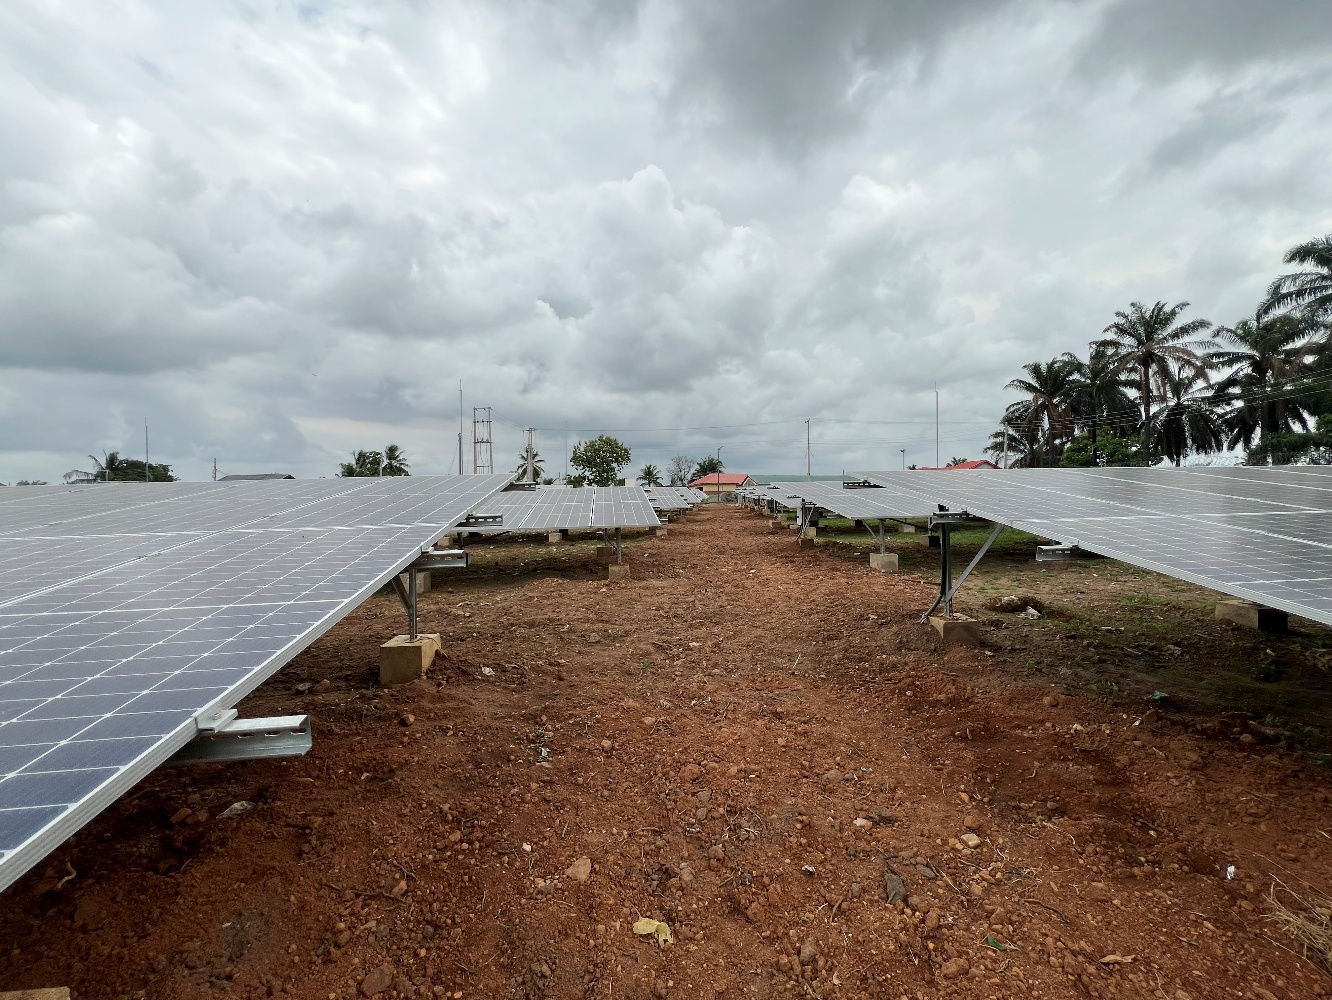
\includegraphics[width=0.6\textwidth]{figures/generation.jpg}
	\caption{Site photo of the solar-mini grid generation plant.}
\end{figure}
\section{Coding Framework: Themes developed during analysis}
\label{app:framework}
\textbf{Theme 1: Carbon Finance Viability (RQ1)}
\begin{itemize}
	\item Awareness and engagement
	\item Transaction costs
	\item Small project scale limitations
	\item Aggregation/PoA mechanisms
	\item Methodology fit and additionality
	\item Revenue potential
	\item Developer motivations
	\item REC alternatives
\end{itemize}

\textbf{Theme 2: Conditions for Scale (RQ2)}
\begin{itemize}
	\item MRV capacity
	\item Baseline and emission factor challenges
	\item Registry and methodological barriers
	\item Policy and licensing uncertainty
	\item NDC and additionality conflicts
	\item Grid arrival risk
	\item Taxation of carbon credits
	\item Financial expectations and capital requirements
\end{itemize}


\bibliographystyle{elsarticle-num} 
\bibliography{references.bib}

\end{document}

\endinput